\documentclass[../norme-di-progetto.tex]{subfiles}

\begin{document}

\subsection{Descrizione}%
\label{sub:processi_primari/descrizione}
Sono i processi essenziali durante il ciclo di vita del software. ISO 12207--1995 ne definisce cinque:

\begin{itemize}
  \item Acquisizione
  \item Fornitura
  \item Sviluppo
  \item Gestione operativa
  \item Manutenzione
\end{itemize}

\subsection{Fornitura}%
\label{sub:fornitura}

\subsubsection{Finalità}%
\label{subs:fornitura/finalita}

GruppOne istanzia il processo di fornitura per potersi aggiudicare il capitolato attraverso un accordo con il committente e la successiva stipulazione di un contratto.

\subsubsection{Descrizione}%
\label{subs:fornitura/descrizione}

Il processo di fornitura contiene le attività e i compiti del fornitore. Esso gestisce il rapporto tra il fornitore e il cliente ed inoltre amministra le procedure e le risorse necessarie per lo sviluppo del piano di progetto. È composto da diverse attività:

\begin{itemize}
  \item Inizializzazione
  \item Preparazione della risposta
  \item Contratto
  \item Pianificazione
  \item Esecuzione e controllo
  \item Revisione e valutazione
  \item Consegna e completamento
\end{itemize}

\subsubsection{Studio di Fattibilità}%
\label{subs:studio_di_fattibilita}
GruppOne si impegna a consegnare un sintetico documento contenente una breve descrizione, i pregi e le criticità riscontrati in ciascuno dei capitolati. Lo studio di fattibilità è redatto dall'\glossario{amministratore}
con l'aiuto degli \glossario{analisti} e ha l'obiettivo di esporre quali capitolati sono stati presi in considerazione con le relative motivazioni. Il documento è così articolato:
\begin{description}
  \item [Descrizione]: si fornisce una breve descrizione del problema esposto dal proponente.
  \item [Finalità del progetto]: si descrive che cosa bisogna realizzare.
  \item [Tecnologie interessate]: si presentano le tecnologie da considerare in fase di sviluppo.
  \item [Aspetti positivi]: si espongono i pregi del capitolato.
  \item [Criticità e fattori di rischio]: si illustrano i difetti osservati studiando il capitolato.
\end{description}

\subsubsection{Incontri con il proponente}%
\label{subs:incontri_con_il_proponente}

Gruppo0ne intende mantenere uno stretto rapporto di collaborazione con i proponenti del capitolato Stalker. Tale rapporto si mantiene attraverso incontri che si svolgono fisicamente presso le aule del Dipartimento di Matematica ``Tullio Levi Civita'' e virtualmente in hangouts.

Gli obiettivi degli incontri sono:
\begin{description}
  \item [Comprensione e perfezionamento dei requisiti]: il team discute col proponente i problemi e i dubbi riscontrati durante l'analisi del capitolato in modo da comprendere incrementalmente i requisiti.
  \item [Ricerca e valutazione del software]: il team chiede al proponente se le componenti e i software proposti soddisfino le funzionalità richieste.
  \item [Convalida dei documenti e del prodotto]: il team si rivolge al proponente per avere conferme sul lavoro svolto siano essi documenti, \glossario{prototipi} appena abbozzati o prodotti software ad uno stato avanzato.
\end{description}
Gli esiti degli argomenti discussi durante gli incontri saranno poi riportati in verbali.

\subsection{Sviluppo}%
\label{sub:sviluppo}

\subsubsection{Finalità}%
\label{subs:sviluppo/finalita}

GruppOne istanzia il processo di sviluppo per realizzare il prodotto richiesto dal proponente.

\subsubsection{Descrizione}%
\label{subs:sviluppo/descrizione}

Il processo di sviluppo contiene le attività e i compiti dello sviluppatore. Esso fissa quali sono gli obiettivi dello sviluppo dalla creazione alla consegna del prodotto finale. Raggruppa le seguenti attività:

\begin{itemize}
  \item Analisi dei requisiti
  \item Progettazione
  \item Codifica
  \item Testing
  \item Installazione
\end{itemize}

\subsubsection{Attività}%
\label{subs:sviluppo/attivita}

\paragraph{Analisi dei requisiti}%
\label{par:analisi_dei_requisiti}
L'analisi dei requisiti è l'attività che studia e comprende il dominio applicativo del problema e che ha come scopo quello di offrire i requisiti che dovranno essere soddisfatti dal software. Si articola nei seguenti compiti:

\begin{itemize}
  \item Studiare e definire il problema da risolvere
  \item Classificare i requisiti
  \item Realizzare i diagrammi UML dei casi d'uso
  \item Ricavare i requisiti atomici da fornire ai progettisti perché possano iniziare l'attività di progettazione
\end{itemize}

Il documento di riferimento, \textit{Analisi dei requisiti v1.0.0}, è redatto dagli analisti.

\subparagraph{Classificazione dei requisiti}%
\label{subp:classificazione_dei_requisiti}

Per identificare i requisiti in maniera univoca, GruppOne ha deciso di adottare delle norme per la classificazione dei requisiti.
Ogni requisito è caratterizzato da un codice alfanumerico così formato:
\begin{center}
  \textbf{R[numero][tipo][priorità]}
\end{center}
in cui ogni elemento ha un diverso significato:
\begin{itemize}
  \item \textbf{Numero}: indica quale numero di caso d'uso si sta esaminando. È un numero progressivo a partire da 1.
  \item \textbf{Tipo}: individua la tipologia di requisito. Esso può essere:
        \begin{itemize}
          \item F:\@funzionale --\@indica servizi che il sistema dovrebbe fornire.
          \item N:\@legislativo --\@indica che le regole che il sistema deve rispettare affinché sia legale.
          \item O:\@organizzativo --\@indica le norme da seguire nel processo di sviluppo:\@ambiente di sviluppo, linguaggio di programmazione o standard di processo.
          \item P:\@prestazionale --\@indica le prestazioni che il programma deve fornire:\@velocità in esecuzione e memoria occupata.
          \item S:\@per la sicurezza --\@indica procedure da adottare affinché il sistema sia considerabile sicuro.
        \end{itemize}
  \item \textbf{Priorità}: determina la priorità del requisito con un numero da 1 a 3:
        \begin{itemize}
          \item 1:\@requisito obbligatorio che deve essere assolutamente soddisfatto dal sistema.
          \item 2:\@requisito desiderabile il cui soddisfacimento è apprezzato dal committente.
          \item 3:\@requisito facoltativo la cui decisione è lasciata al team.
        \end{itemize}
\end{itemize}
\subparagraph{Casi d'uso}%
\label{subp:casi_d'uso}
I diagrammi dei casi d'uso descrivono le funzioni e i servizi offerti dal prodotto agli attori che interagiscono con il sistema. Ogni caso d'uso ha:

\begin{itemize}
  \item Una rappresentazione testuale
  \item Una rappresentazione grafica
\end{itemize}

Nel presente paragrafo si descrive la rappresentazione testuale mentre nel successivo verrà descritta la rappresentazione grafica. Un generico caso d'uso è caratterizzato da:
\begin{description}
  \item [Sigla del caso d`uso]: per avere più ordine nell'esposizione dei casi d'uso si antepone una lettera maiuscola al caso d'uso. Useremo:
  \begin{itemize}
   \item --A per distinguere i casi d'uso dell'admin.
   \item --U per distinguere i casi d'uso utente.
  \end{itemize}
  \item [Titolo]: breve titolo del caso d'uso.
  \item [Codice]: codice identificativo del caso d'uso. Ogni caso d'uso può essere suddiviso in altri sottocasi. La denominazione convenzionale è la seguente:
        \begin{description}
          \item [Caso d'uso]: [A/U]UC[codice numerico].
          \item [Sottocaso d'uso]: [A/U]UC[codice numerico del padre].[codice numerico del sottocaso].
        \end{description}
        Ad esempio il primo caso d'uso admin avrà codice identificativo AUC1 mentre i relativi sottocasi saranno AUC1.1 AUC1.2 AUC1.3..
  \item [Attore primario]: attore principale coinvolto nel caso d'uso.
  \item [Attori secondari (opzionale)]: attori secondari coinvolti nel caso d'uso.
  \item [Precondizione]: condizione in cui si trovano gli attori prima del verificarsi del caso d'uso.
  \item [Postcondizione]: condizione in cui si trovano gli attori dopo il verificarsi del caso d'uso.
  \item [Scenario principale]: sequenza di azioni svolte dall'attore per portare a compimento il caso d'uso.
  \item [Inclusioni (opzionale)]: il caso d'uso incluso è incondizionatamente eseguito dal caso d'uso che lo include.
  \item [Estensioni (opzionale)]: sequenza di possibilità dell'attore al verificarsi di eventi anomali o di situazioni di errore.
\end{description}

\subparagraph{Diagrammi UML dei casi d'uso}%
\label{subp:diagrammi_UML_dei_casi_d'uso}
I diagrammi dei casi d'uso forniscono una rappresentazione grafica del caso d'uso che si sta descrivendo. Purtroppo non danno alcun tipo di valore aggiunto alla rappresentazione testuale dato che non possono descrivere precondizioni e postcondizioni. I principali elementi di un diagramma UML sono:
\begin{itemize}
  \item Attori
  \item Scenario
  \item Use case
\end{itemize}
Gli attori interagiscono con il sistema pertanto si trovano fuori dallo scenario, mentre gli use case sono parte integrante dello scenario. I collegamenti tra attori e casi d'uso e tra quest'ultimi e altri casi d'uso avvengono tramite legami rappresentati mediante linee. Possono essere di quattro differenti tipi:
\begin{description}
  \item [Associazione]: l'associazione è la comunicazione diretta tra attore e use case. Rappresenta la partecipazione dell'attore al caso d'uso a cui è legato.
  \item [Inclusione]: L'inclusione è un legame diretto stretto tra due use case. Dati due casi d'uso A e B, si dice che A include B se ogni istanza di A esegue B. B è incluso nell'esecuzione di A e la responsabilità di esecuzione di B è unicamente di A.
  \item [Estensione]: L'estensione aumenta le funzionalità di uno use case. Dati due casi d'uso A e B, si dice che B estende A se A esegue B solo a determinate condizioni. L'esecuzione di B interrompe A e per questo motivo viene utilizzata prevalentemente per gestire errori e eccezioni.
  \item [Generalizzazione]: La generalizzazione è un legame tra attori o più raramente tra use case. Dati due casi d'uso A e B, A è generalizzazione di B se condivide almeno le funzionalità di A. B può modificare le funzionalità di A, mentre tutte le funzionalità non ridefinite si mantengono identiche a quelle di A.
\end{description}

\paragraph{Progettazione}%
\label{par:progettazione}
L'attività di progettazione si occupa di organizzare le componenti del sistema determinandone la struttura. Essa procede inversamente rispetto all'analisi dei requisiti la quale adotta un approccio investigativo, di studio del dominio applicativo e di scomposizione dei requisiti. La progettazione cerca, invece, di fissare l'architettura del prodotto scegliendo una soluzione che possa soddisfare tutti gli \glossario{stakeholders}.
Essa si pone i seguenti obiettivi:
\begin{itemize}
  \item Soddisfare i requisiti con un sistema di qualità.
  \item Ricercare una buona soluzione architetturale.
  \item Suddividere il problema in sotto-problemi più semplici da risolvere.
\end{itemize}

\subparagraph{Technology Baseline}%
\label{subp:technology_baseline}
La \glossario{technology baseline} è un documento parte integrante della RP.\@ Essa presenta:

\begin{itemize}
  \item Le tecnologie
  \item I framework
  \item Le librerie
\end{itemize}
Deve contenere inoltre una \glossario{proof of concept} che ha lo scopo di evidenziare come le tecnologie utilizzate possano servire allo sviluppo del prodotto.

\subparagraph{Product Baseline}%
\label{subp:product_baseline}
La \glossario{product baseline} è un documento parte integrante della RQ.\@ Ha il compito di mostrare l'architettura del prodotto attraverso la creazione di:

\begin{itemize}
  \item Diagrammi delle classi
  \item Diagrammi di sequenza
  \item Diagrammi delle attività
  \item Diagrammi di package
\end{itemize}

\subsubsection{Strumenti}%
\label{subs:strumenti}

\paragraph{PlantUml}%
\label{par:plantuml}
Per la costruzione dei diagrammi dei casi d'uso il team ha deciso di utilizzare PlantUml. È un software open source che permette la costruzione di diagrammi UML a partire dalla scrittura di codice. PlantUml fa uso di GraphViz per la traduzione del plain text in elementi grafici. GruppOne ha valutato positivamente tale strumento in quanto:

\begin{itemize}
  \item Permette di scrivere i diagrammi dei casi d'uso sotto forma di codice, mentre il ruolo di costruzione dei diagrammi è demandato al software sottostante.
  \item Permette di scrivere agevolmente non solo i diagrammi dei casi d'uso, ma anche diagrammi delle classi, di sequenza e di package.
\end{itemize}

\begin{figure}[H]
  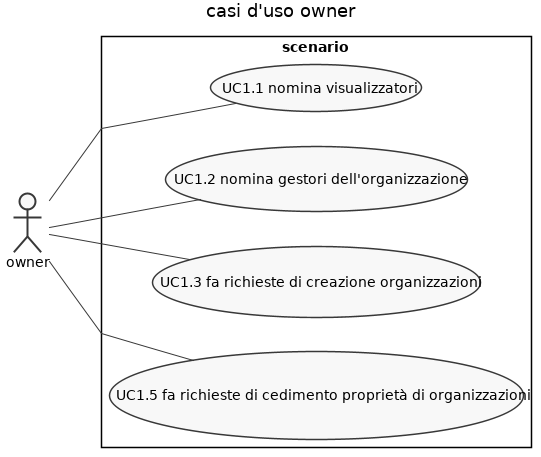
\includegraphics[width=8cm]{components/img/owner_use_cases.png}
  \centering
  \caption{diagramma dei casi d'uso realizzato con PlantUml}
\end{figure}

\end{document}
